\section{2D EQUATIONS OF MOTION}

\begin{whitebox}{}
    \begin{tabularx}{\columnwidth}{lclclc}
        $T$ & $\unit{N}$ & Thrust force\\
        $m$ & $\unit{kg}$ & Mass\\
        $g$ & $\unit{m.s^{-2}}$ & Gravitational accel. & $9.80665\ \unit{m.s^{-2}}$\\
        $\gamma$ & $\unit{rad}$ & Flight path angle\\
        %$\bar{\gamma}$ & $\unit{rad}$ & Glide angle\\
        $\alpha$ & $\unit{rad}$ & Angle of attack\\
        $\sigma$ & $\unit{rad}$ & Thrust incidence angle\\
        $V_C$ & $\unit{m.s^{-1}}$ & Climb speed\\
        $V_S$ & $\unit{m.s^{-1}}$ & Sink speed\\
        $V_H$ & $\unit{m.s^{-1}}$ & Horizontal speed\\
    \end{tabularx}
\end{whitebox}

\resizebox{1.0\linewidth}{!}{
    \includegraphics[
    page = {14},
    trim = {6.0cm, 7.7cm, 6.0cm, 3.8cm}, % left, bottom, right, top
    clip
    ]{Lecture01.pdf}
}

\begin{highlightbox}{\textbf{GENERAL 2D EQUATIONS OF MOTION}}
    \begin{align}
        \label{eq:2d_eom_x}
        (x) \quad &m\dot{V}=T\cos(\alpha+\sigma)-D-mg\sin\gamma\\
        \label{eq:2d_eom_y}
        (y) \quad &mV\dot{\gamma}=L+T\sin(\alpha+\sigma)-mg\cos\gamma
    \end{align}
\end{highlightbox}

\begin{highlightbox}{\textbf{HORIZONTAL \& VERTICAL SPEED}}
    \begin{align}
        \label{eq:2d_eom_horizspeed}
        &V_H=V\cos\gamma\\
        \label{eq:2d_eom_vertspeed}
        &V_C=V_S=V\sin\gamma
    \end{align}
\end{highlightbox}

\begin{whitebox}{\textbf{STATIONARY GLIDING FLIGHT}}
    \blue{Conditions}
    \begin{itemize}
        \item $T=0$
        \item $\sfrac{d(\cdot)}{dt}=0$
    \end{itemize}
    
    \blue{Assumptions}
    \begin{itemize}
        \item $\alpha\approx 0$
        \item $\sigma\approx0$
    \end{itemize}
    
    \begin{highlightbox}{}
        \begin{align}
            \label{eq:stat_glide_drag}
            &D=mg\sin\gamma\\
            \label{eq:stat_glide_lift}
            &L=mg\cos\gamma
        \end{align}
    \end{highlightbox}

    \centering
    \resizebox{0.6\linewidth}{!}{
        \includegraphics[
        page = {25},
        trim = {10.5cm, 1.0cm, 4.5cm, 8.5cm}, % left, bottom, right, top
        clip
        ]{Lecture01.pdf}
    }
    \resizebox{1.0\linewidth}{!}{
        \includegraphics[
        page = {28},
        trim = {1.0cm, 5.5cm, 6.5cm, 2.5cm}, % left, bottom, right, top
        clip
        ]{Lecture01.pdf}
    }

    \mathbox{
        \frac{V_H}{V_S}=\frac{L}{D}\overset{\scriptscriptstyle\eqref{eq:lift},\eqref{eq:drag}}{=}\frac{c_L}{c_D}=\frac{1}{\tan\gamma}\overset{\gamma\ll1}{\approx}\frac{1}{\gamma}
    }
    
    \mathbox{
        \tan(\gamma_{\min})=\frac{1}{\left(\frac{c_L}{c_D}\right)_{\max}}
    }
    
    \mathbox{
        V\overset{\scriptscriptstyle\eqref{eq:lift}}{=}\sqrt{\frac{2mg}{\rho S_{ref}c_L}\cos\gamma}\overset{\gamma\ll1}{\approx}\sqrt{\frac{2mg}{\rho S_{ref}c_L}}
    }
    
    \mathbox{
        V_S=\sqrt{\frac{2mg}{\rho S_{ref}}\frac{c_D^2}{c_L^3}\cos^3(\gamma)} \overset{\gamma\ll1}{\approx}\sqrt{\frac{2mg}{\rho S_{ref}}\frac{c_D^2}{c_L^3}}
    }
    
    \mathbox{
        V_H=\sqrt{V^2-V_S^2}
    }
    
    \mathbox{
        V_{H,\min}\overset{\gamma\ll1}{\approx}V(c_L=c_{L,\max})
    }
    
    \mathbox{
        V_{S,\min}\overset{\gamma\ll1}{\approx}V_S\left(\left(\frac{c_L^3}{c_D^2}\right)_{\max}\right)
    }

\end{whitebox}